\documentclass{report}
\usepackage[english]{babel}

\usepackage[most,many,breakable]{tcolorbox}
\usepackage{xcolor}

\definecolor{defBoxBorder}{HTML}{395144}
\newtcolorbox{defBox}{colback=white,colframe=defBoxBorder,arc=3pt, boxrule=0.5pt, drop fuzzy shadow, title=Definition}
\definecolor{thBoxBorder}{HTML}{AC8441}
\newtcolorbox{thBox}{colback=white,colframe=thBoxBorder,arc=3pt, boxrule=0.5pt, drop fuzzy shadow, title=Theorem}
\definecolor{noteBoxBorder}{HTML}{4E6C50}
\newtcolorbox{noteBox}{colback=white,colframe=noteBoxBorder,arc=3pt, boxrule=0.5pt, drop fuzzy shadow, title=Note}
\definecolor{axBoxBorder}{HTML}{AA5656}
\newtcolorbox{axBox}{colback=white,colframe=axBoxBorder,arc=3pt, boxrule=0.5pt, drop fuzzy shadow, title=Axiom/Postulate}
\definecolor{corBoxBorder}{HTML}{8B7E74}
\newtcolorbox{corBox}{colback=white,colframe=corBoxBorder,arc=3pt, boxrule=0.5pt, drop fuzzy shadow, title=Corollary}
\definecolor{lemBoxBorder}{HTML}{B99B6B}
\newtcolorbox{lemBox}{colback=white,colframe=lemBoxBorder,arc=3pt, boxrule=0.5pt, drop fuzzy shadow, title=Lemma}
\definecolor{asBoxColor}{HTML}{FDFDF9}
\definecolor{asBoxBorder}{HTML}{DEB881}
\newtcolorbox{asBox}{coltext=black, colback=asBoxColor,colframe=asBoxBorder,arc=3pt, boxrule=0.5pt, drop fuzzy shadow, title=Aside}


\input{setup.tex}

\begin{document}
    \coverPage{Matemáticas}{Cálculo Diferencial}{Límites y Continuidad}{}{Alexander Mendoza}{\today}
    \tableofcontents

    \tikzset{every picture/.style={line width=0.75pt}} % establecer el ancho de línea predeterminado en 0.75pt
    \pagebreak
    \chapter{Límites}

    \section{Un enfoque intuitivo de los límites}
    Cuando hablamos de cálculo, lo primero que nos viene a la mente son las derivadas e integrales; sin embargo, la idea más fundamental de esta disciplina es la noción de límites. Comencemos definiendo los límites de una manera intuitiva. Decimos que el límite de $f(x)$ cuando $x$ se acerca a $a$ (se acerca a $a$) es $L$ si los valores de $f$ pueden acercarse tanto como deseemos a $L$ siempre que $x$ esté suficientemente cerca, pero diferente de $a$.

    Un límite implica dos cosas: una función $f(x)$ y un punto $a$ en el cual analizaremos la función. Este concepto de "análisis" de la función se refiere a una revisión específica del comportamiento de la función para valores cercanos a $a$. Sabiendo esto, no podemos hablar de límites de una manera general, la definición de límites solo se aplica a un punto particular.

    \begin{Figure}
        \begin{center}
            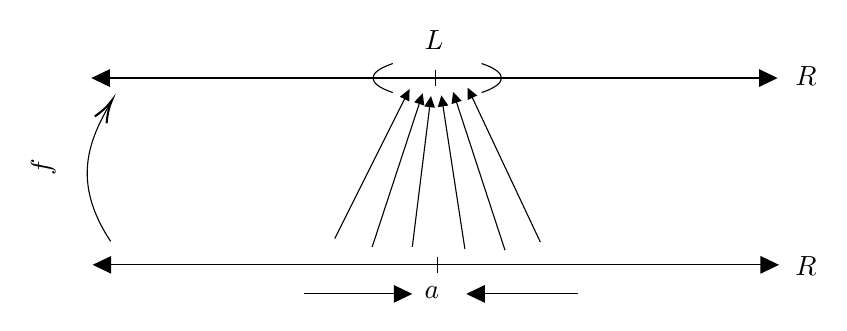
\begin{tikzpicture}[x=0.75pt,y=0.75pt,yscale=-1,xscale=1]
            %uncomment if require: \path (0,459); %set diagram left start at 0, and has height of 459
            %Curve Lines [id:da05569855742087637] 
            \draw    (108.67,199) .. controls (89.27,169.9) and (98.72,149.58) .. (108.43,132.57) ;
            \draw [shift={(109.33,131)}, rotate = 119.98] [color={rgb, 255:red, 0; green, 0; blue, 0 }  ][line width=0.75]    (10.93,-3.29) .. controls (6.95,-1.4) and (3.31,-0.3) .. (0,0) .. controls (3.31,0.3) and (6.95,1.4) .. (10.93,3.29)   ;
            %Straight Lines [id:da4013382751057579] 
            \draw    (103,210.33) -- (427.67,210.33) (266,206.33) -- (266,214.33) ;
            \draw [shift={(430.67,210.33)}, rotate = 180] [fill={rgb, 255:red, 0; green, 0; blue, 0 }  ][line width=0.08]  [draw opacity=0] (8.93,-4.29) -- (0,0) -- (8.93,4.29) -- cycle    ;
            \draw [shift={(100,210.33)}, rotate = 0] [fill={rgb, 255:red, 0; green, 0; blue, 0 }  ][line width=0.08]  [draw opacity=0] (8.93,-4.29) -- (0,0) -- (8.93,4.29) -- cycle    ;
            %Straight Lines [id:da6399022660258387]
            \draw    (102.33,120.33) -- (427,120.33) (265.33,116.33) -- (265.33,124.33) ;
            \draw [shift={(430,120.33)}, rotate = 180] [fill={rgb, 255:red, 0; green, 0; blue, 0 }  ][line width=0.08]  [draw opacity=0] (8.93,-4.29) -- (0,0) -- (8.93,4.29) -- cycle    ;
            \draw [shift={(99.33,120.33)}, rotate = 0] [fill={rgb, 255:red, 0; green, 0; blue, 0 }  ][line width=0.08]  [draw opacity=0] (8.93,-4.29) -- (0,0) -- (8.93,4.29) -- cycle    ;
            %Shape: Output [id:dp34058752983845664]
            \draw   (244.6,113.33) .. controls (231.86,117.66) and (231.86,123) .. (244.6,127.33) (194.67,120.33) -- (234.61,120.33) (337.33,120.33) -- (297.39,120.33) (287.4,113.33) .. controls (300.14,117.66) and (300.14,123) .. (287.4,127.33) ;
            %Straight Lines [id:da412096367731386]
            \draw    (216.67,197.67) -- (251.33,128.35) ;
            \draw [shift={(252.67,125.67)}, rotate = 116.57] [fill={rgb, 255:red, 0; green, 0; blue, 0 }  ][line width=0.08]  [draw opacity=0] (5.36,-2.57) -- (0,0) -- (5.36,2.57) -- cycle    ;
            %Straight Lines [id:da8178341794483637]
            \draw    (315.67,199.33) -- (281.94,127.71) ;
            \draw [shift={(280.67,125)}, rotate = 64.79] [fill={rgb, 255:red, 0; green, 0; blue, 0 }  ][line width=0.08]  [draw opacity=0] (5.36,-2.57) -- (0,0) -- (5.36,2.57) -- cycle    ;
            %Straight Lines [id:da12457344272068971]
            \draw    (298.67,203.33) -- (274.6,129.85) ;
            \draw [shift={(273.67,127)}, rotate = 71.87] [fill={rgb, 255:red, 0; green, 0; blue, 0 }  ][line width=0.08]  [draw opacity=0] (5.36,-2.57) -- (0,0) -- (5.36,2.57) -- cycle    ;
            %Straight Lines [id:da23360491003650297]
            \draw    (234.67,201.67) -- (258.06,130.52) ;
            \draw [shift={(259,127.67)}, rotate = 108.2] [fill={rgb, 255:red, 0; green, 0; blue, 0 }  ][line width=0.08]  [draw opacity=0] (5.36,-2.57) -- (0,0) -- (5.36,2.57) -- cycle    ;
            %Straight Lines [id:da4317804152860907]
            \draw    (254,201.67) -- (262.63,131.98) ;
            \draw [shift={(263,129)}, rotate = 97.06] [fill={rgb, 255:red, 0; green, 0; blue, 0 }  ][line width=0.08]  [draw opacity=0] (5.36,-2.57) -- (0,0) -- (5.36,2.57) -- cycle    ;
            %Straight Lines [id:da9892035418701624]
            \draw    (279.33,202.67) -- (268.45,131.63) ;
            \draw [shift={(268,128.67)}, rotate = 81.29] [fill={rgb, 255:red, 0; green, 0; blue, 0 }  ][line width=0.08]  [draw opacity=0] (5.36,-2.57) -- (0,0) -- (5.36,2.57) -- cycle    ;
            %Straight Lines [id:da35085103715970445]
            \draw    (202,224.33) -- (251,224.33) ;
            \draw [shift={(254,224.33)}, rotate = 180] [fill={rgb, 255:red, 0; green, 0; blue, 0 }  ][line width=0.08]  [draw opacity=0] (8.93,-4.29) -- (0,0) -- (8.93,4.29) -- cycle    ;
            %Straight Lines [id:da8736603322533996]
            \draw    (334,224.33) -- (283,224.33) ;
            \draw [shift={(280,224.33)}, rotate = 360] [fill={rgb, 255:red, 0; green, 0; blue, 0 }  ][line width=0.08]  [draw opacity=0] (8.93,-4.29) -- (0,0) -- (8.93,4.29) -- cycle    ;
            % Text Node
            \draw (437.33,113.67) node [anchor=north west][inner sep=0.75pt]    {$\mathbb{R}$};
            % Text Node
            \draw (437.33,205.33) node [anchor=north west][inner sep=0.75pt]    {$\mathbb{R}$};
            % Text Node
            \draw (68.95,168.59) node [anchor=north west][inner sep=0.75pt]  [rotate=-270.38]  {$f$};
            % Text Node
            \draw (258.67,219.67) node [anchor=north west][inner sep=0.75pt]    {$a$};
            % Text Node
            \draw (258.67,96.33) node [anchor=north west][inner sep=0.75pt]    {$L$};
            \end{tikzpicture}
        \end{center}
    \end{Figure}

    Como se puede ver en la Figura 1.1.1, a medida que nos acercamos a $a$, $f(x)$ se acerca a $L$. En los límites, debemos acercarnos tanto como deseemos a $L$, esto es posible debido a la continuidad de $\mathbb{R}$.

    \chapter{Continuidad}

    \section{Funciones continuas}

    Aunque en muchos casos, dado una función arbitraria $f$, $\lim_{x \to a} f(x) = f(a)$, no siempre es el caso. Por ejemplo, sea $f$ una función tal que
    $$f(x) = \begin{cases}
        1 & \text{si } x = 0\\
        x & \text{si } x \neq 0
    \end{cases}$$

    Entonces está claro que $\lim_{x \to 0} f(x) = 0$ y $f(0) = 1$. Las funciones donde el límite en un punto $a$ es igual a la función evaluada en ese mismo punto $a$ son muy particulares y se llaman funciones continuas. La idea intuitiva de funciones continuas es una función que, cuando miramos su gráfica, no tiene espacios, saltos ni cambios bruscos. Como sabemos, definir cosas desde un punto de vista intuitivo puede ser problemático, por eso la definición formal de funciones continuas es la siguiente:\\

    \begin{defBox}
        Una función $f$ es continua en $a$ si el límite de $f(x)$ cuando $x$ se acerca a $a$ existe, $f$ está definida en $a$ y $$\lim_{x \to a}f(x) = f(a)$$
    \end{defBox}

    Revisemos algunas funciones comunes y veamos si son continuas.

    \begin{Example}
        $f(x) = c$ para alguna constante $c \in \mathbb{R}$. Esta función es, de hecho, continua. $\lim_{x \to a}f(x) = c = f(a)$, esto se debe a las propiedades de límites de una función constante.
    \end{Example}

    \begin{Example}
        $f(x) = ax+b$ para algunos $a, b \in \mathbb{R}$. Esta función también es continua. $\lim_{x \to a}f(x) = a = f(a)$, esto se debe a las propiedades de límites de la función identidad.
    \end{Example}

    \begin{Example}
        $f(x) = a_nx^n + a_{n-1}x^{n-1}+\cdots + a_1x_1 + a_0$ (polinomio de grado $n$). Cualquier función polinómica es continua.
    \end{Example}

    \begin{Example}
        $f(x) = \dfrac{p(x)}{q(x)}$ donde $p(x)$ y $q(x)$ son polinomios y $q(x) \neq 0$ también es una función continua.
    \end{Example}

    \begin{Example}
        $f(x) = \sin x$ y $g(x) = \cos x$. También son funciones continuas.
    \end{Example}

    Junto con esta definición, también surge el siguiente teorema.\\

    \begin{thBox}
        Sean $f$ y $g$ funciones continuas en $x=a$, entonces tenemos que:

        \begin{enumerate}
            \item $f+g$ también es continua en $a$.
            \item $f \cdot g$ también es continua en $a$.
            \item $\frac{1}{g}$ también es continua en $a$ si $g(a) \neq 0$.
        \end{enumerate}
    \end{thBox}

    \textit{\textbf{Demostración.}} Probaremos la propiedad 1 y las demás siguen una idea similar. Sean $f$ y $g$ funciones continuas en $x=a$, entonces

    $$
        \lim_{x\to a} f(x) = f(a) \text{ y } \lim_{x\to a} g(x) = g(a)
    $$

    Con esto y el teorema de límites, tenemos que

    $$
        \lim_{x \to a} (f+g)(x) = f(a) + g(a) = (f+g)(a)
    $$

    También hay otra propiedad importante que dicta cómo se comporta la continuidad en las composiciones de funciones.\\

    \begin{thBox}
        Si $f$ es continua en $g(a)$ y $g$ es continua en $a$, entonces $f \circ g$ es continua en $a$.
    \end{thBox}
\end{document}
